\documentclass[10pt]{article}
\usepackage[margin=0.78in]{geometry}
\usepackage{amsmath,amssymb,amsthm,booktabs,graphicx,microtype,placeins}
\usepackage[font=small,skip=3pt]{caption}
\usepackage[hidelinks]{hyperref}
\setlength{\parindent}{0pt}
\setlength{\parskip}{3pt plus 1pt minus 1pt}
\setlength{\textfloatsep}{7pt plus 2pt minus 2pt}
\setlength{\intextsep}{7pt plus 2pt minus 2pt}
\newtheorem{theorem}{Theorem}
\newtheorem{proposition}[theorem]{Proposition}
\theoremstyle{definition}
\newtheorem{definition}[theorem]{Definition}
\title{\vspace{-1.7em}\textbf{Semantic Structure Predicts}\\[-1pt]
\textbf{Exact Boolean Formula Complexity}}
\author{J. R. Landers}
\date{\vspace{-1.4em}}

\begin{document}
\maketitle
\vspace{-1.6em}

\begin{abstract}
We ask how much exact Boolean formula complexity is predictable from function
semantics rather than formula syntax.  Every one of the 65,536 four-input
Boolean functions is synthesized exactly in NAND, NOR, and AND/OR/NOT formula
languages.  A tie-aware nearest-neighbor model uses only truth-table
invariants: signed bias, sorted influences, Walsh--Fourier energy by degree,
algebraic degree, and input-permutation stabilizer size.  After removing every
training function with the test descriptor, the model explains $77.7\%$,
$77.7\%$, and $84.3\%$ of exact minimum-size variance in the three languages.
The best descriptor-measurable predictions explain $89.3\%$, $89.3\%$, and
$93.1\%$, respectively.  No matched permutation reaches an observed result
($p=1/1001<0.001$).  An order-invariant reanalysis of all 256 three-input
functions yields lower strict values of $53.8\%$, $53.8\%$, and $58.9\%$;
the four-input result is stable across neighbor thresholds and coordinate
scalings.  Elementary semantics therefore contains substantial, scalable
information about exact representation cost, while imperfect cross-language
rank stability confirms that cost is not intrinsic to the function alone.
\end{abstract}

\section{Problem and formal setup}

\textbf{Takeaway.} Meaning strongly correlates with and predicts representation
cost, but does not completely dictate it: even the full descriptor leaves a
nonzero within-class residual, and the chosen gate language still matters.

Let $\mathcal B_n=\{f:\{0,1\}^n\to\{0,1\}\}$, with $n\in\{3,4\}$.
A formula language $\mathcal L$ consists of variables $x_0,\ldots,x_{n-1}$ and
a fixed gate basis.  Formulas are rooted trees, and size $|e|$ is the number of
gates.  This basis-relative notion descends from classical switching synthesis
\cite{shannon1949} and remains central in modern exact synthesis
\cite{haaswijk2020,panchu2023}.

\begin{definition}[Exact formula complexity]
For evaluation map $\operatorname{eval}_{\mathcal L}:E_{\mathcal L}\to
\mathcal B_n$, define
\[
 K_{\mathcal L}(f)=\min\{|e|:
 \operatorname{eval}_{\mathcal L}(e)=f\}.
 \tag{1}
\]
\end{definition}

The three languages are NAND, NOR, and ordered AND/OR/NOT.  They are
functionally complete but assign different costs to the same truth table.
For $f\in\mathcal B_n$, let
\[
 \psi_n(f)=\bigl(b(f),\operatorname{sort}(I_1(f),\ldots,I_n(f)),
 E_0(f),\ldots,E_n(f),\deg_{\mathbb F_2}(f),|\operatorname{Stab}(f)|\bigr)
 \in\mathbb R^{2n+4}.
 \tag{2}
\]
Here $b$ is signed output bias, $I_i$ is variable influence, $E_d$ is
Walsh--Fourier energy at degree $d$, and the stabilizer is under input
permutations.  These are computed from the truth table and contain no gate or
formula data.  Influence and Fourier summaries have classical connections to
circuit structure and learnability \cite{lmn1993,odonnell2014}; O'Donnell and
Servedio directly relate influence to decision-tree size
\cite{odonnellservedio2007}.

\begin{proposition}[Input-renaming invariance]
For every $\pi\in S_n$, language $\mathcal L$, and function $f$,
\[
 K_{\mathcal L}(f\circ\pi)=K_{\mathcal L}(f),
 \qquad \psi_n(f\circ\pi)=\psi_n(f).
 \tag{3}
\]
\end{proposition}
\begin{proof}
Relabeling every leaf is a size-preserving bijection of formulas.  Bias,
sorted influences, Fourier energy by degree, algebraic degree, and stabilizer
cardinality are coordinate-permutation invariants.
\end{proof}

\section{Exact synthesis}

Let $M_\ell\subseteq\mathcal B_n$ be the functions whose minimum formula size
is exactly $\ell$, with $M_0$ the variable truth tables.  If $\mathcal O_r$ is
the set of $r$-ary gates, define the candidate layer
\[
 R_\ell=\bigcup_{r\ge1}\ \bigcup_{o\in\mathcal O_r}\
 \bigcup_{\ell_1+\cdots+\ell_r=\ell-1}
 \{o(f_1,\ldots,f_r):f_j\in M_{\ell_j}\}.
 \tag{4}
\]

\begin{theorem}[Minimum-layer recurrence]
For every $\ell\ge1$,
\[
 M_\ell=R_\ell\setminus\bigcup_{j<\ell}M_j.
 \tag{5}
\]
Consequently, the first layer containing $f$ gives $K_{\mathcal L}(f)$ exactly.
\end{theorem}
\begin{proof}
Every size-$\ell$ formula has a root gate and subformula sizes summing to
$\ell-1$.  In a minimum formula, each subformula must itself be minimum for
the function it computes; otherwise replacing it would shorten the whole
formula.  Thus every minimum formula occurs in $R_\ell$, and removing earlier
layers leaves precisely the new minima.  The reverse inclusion follows by
construction.
\end{proof}

Vectorized evaluation of (5) reaches every four-input truth table.  As
independent checks, the implementation reproduces all previously counted
three-input minima and verifies the all-function duality
$K_{\rm NAND}(f)=K_{\rm NOR}(\neg f(\neg x))$.  Table~\ref{tab:scale}
summarizes the complete universes.

\begin{table}[!htbp]
\centering\small
\begin{tabular}{lrrrr}
\toprule
Universe & Functions & $S_n$ orbits & Descriptor classes & Maximum minima \\
\midrule
$n=3$ & 256 & 80 & 36 & NAND/NOR 14 \\
$n=4$ & 65,536 & 3,984 & 675 & NAND/NOR 26; A/O/N 19 \\
\bottomrule
\end{tabular}
\caption{Complete synthesis scale.  Four-input mean minima are 12.231 gates
for NAND/NOR and 10.141 for AND/OR/NOT.}
\label{tab:scale}
\end{table}

\section{Prediction and falsification protocol}

Descriptor coordinates are standardized.  For a test function $f$, let
$T(f)$ be the permitted training functions and let $r_k(f)$ be the distance to
its $k$th nearest member.  To remove arbitrary truth-table ordering when
distances tie, define
\[
 N_k^\ast(f)=\{g\in T(f):\|\psi_n(g)-\psi_n(f)\|_2\le r_k(f)\},
 \qquad
 \widehat K_{\mathcal L}(f)=\frac{1}{|N_k^\ast(f)|}
 \sum_{g\in N_k^\ast(f)}K_{\mathcal L}(g),
 \tag{6}
\]
with $k=7$.  Thus at least seven neighbors are used, including the complete
boundary tie shell.

Three nested protocols remove (i) only $f$; (ii) the complete $S_n$ orbit of
$f$; or (iii) the complete descriptor fiber
$\psi_n^{-1}(\psi_n(f))$.  The strict protocol therefore contains neither an
input-renamed copy nor any function with the same descriptor.  Performance is
\[
 R^2=1-\frac{\sum_f(K_{\mathcal L}(f)-\widehat K_{\mathcal L}(f))^2}
 {\sum_f(K_{\mathcal L}(f)-\overline K_{\mathcal L})^2}.
 \tag{7}
\]

The descriptor ceiling predicts each function by its descriptor-class mean.
It is the largest possible $R^2$ for a predictor measurable only with respect
to these exact classes, since the class mean minimizes within-class squared
error.  The matched null preserves signed bias, algebraic degree, and
stabilizer size.  Within each exact stratum $z$, complexity labels are
permuted and the fixed strict plan is reevaluated, testing
\[
 H_0:K_{\mathcal L}\ \perp\!\!\!\perp\ \psi_n\mid z,
 \qquad
 p=\frac{1+\#\{b:R_b^2\ge R_{\rm obs}^2\}}{B+1},\quad B=1000.
 \tag{8}
\]
The plus-one correction prevents zero Monte Carlo $p$-values
\cite{phipson2010}.

\section{Results}

The main result is the descriptor-held-out column of
Table~\ref{tab:main}.  Semantics explains $77.7\%$ of exact NAND/NOR variance
and $84.3\%$ of AND/OR/NOT variance without an exact semantic twin in training.

\begin{table}[!htbp]
\centering\small
\begin{tabular}{lrrrrrr}
\toprule
Language & Function $R^2$ & Orbit $R^2$ & Strict $R^2$ & Ceiling $R^2$ & RMSE & Null 95\% \\
\midrule
NAND       & .890 & .851 & .777 & .893 & 1.505 & $[.038,.048]$ \\
NOR        & .890 & .851 & .777 & .893 & 1.505 & $[.038,.048]$ \\
AND/OR/NOT & .929 & .906 & .843 & .931 & 1.031 & $[.047,.056]$ \\
\bottomrule
\end{tabular}
\caption{Four-input prediction.  No matched permutation reaches an observed
strict result, so $p=1/1001<0.001$ in every language.}
\label{tab:main}
\end{table}

\begin{figure}[!htbp]
\centering
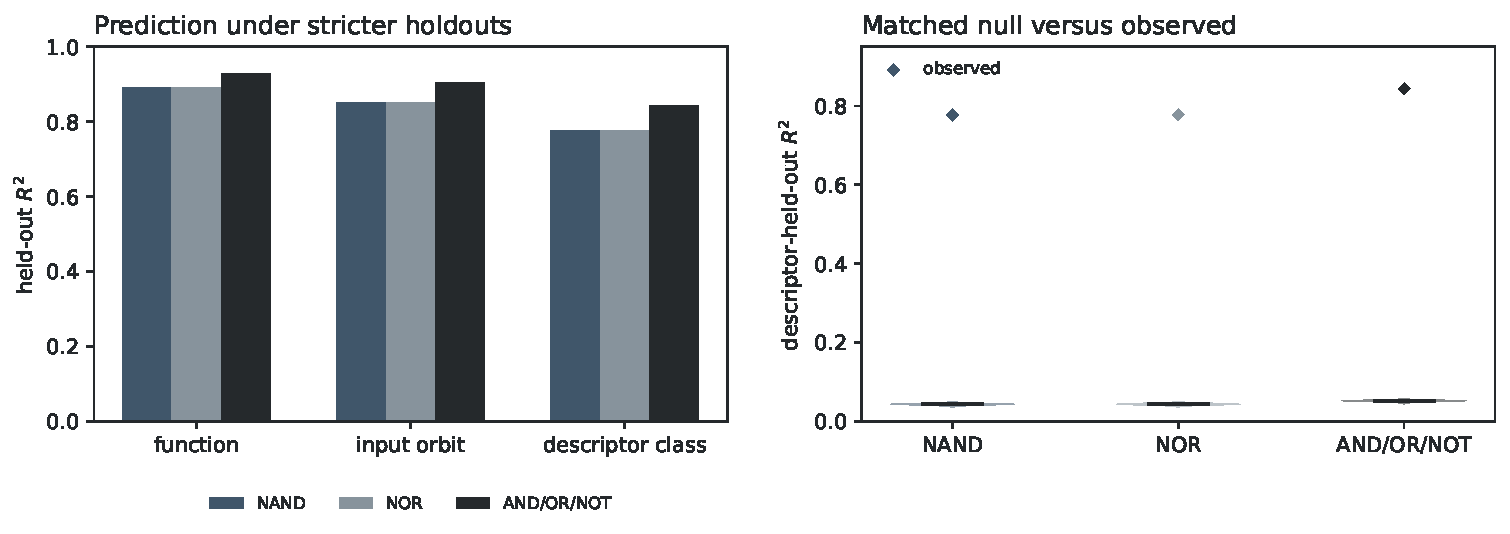
\includegraphics[width=0.98\textwidth]{../../experiments/semantic-boolean-complexity-4bit/figures/four_bit_validation.pdf}
\caption{Leakage and null controls.  Prediction attenuates under stricter
holdouts (left), yet strict observations remain far above bias/degree/symmetry-
matched permutation distributions (right).}
\label{fig:validation4}
\end{figure}
\FloatBarrier

The same tie-aware protocol on three inputs gives strict $R^2$ values .538,
.538, and .589, compared with .777, .777, and .843 at four inputs.  Thus the
stronger signal is not an artifact of changing the tie rule.  Table
\ref{tab:ablation} shows that bias, degree, and symmetry alone carry essentially
no strict predictive power, whereas influence and Fourier coordinates are
independently informative.

\begin{table}[!htbp]
\centering\small
\begin{tabular}{lrrr}
\toprule
Features & NAND $R^2$ & NOR $R^2$ & AND/OR/NOT $R^2$ \\
\midrule
Bias, degree, symmetry & .002 & .002 & $-.059$ \\
Influences only        & .669 & .669 & .819 \\
Fourier energy only    & .666 & .666 & .828 \\
Without influences     & .637 & .637 & .636 \\
Without Fourier        & .791 & .791 & .806 \\
Full descriptor        & .777 & .777 & .843 \\
\bottomrule
\end{tabular}
\caption{Four-input descriptor ablations under strict holdout.  The slight
NAND/NOR gain after removing Fourier coordinates indicates Euclidean-distance
dilution, not absence of Fourier signal.}
\label{tab:ablation}
\end{table}

\begin{figure}[!htbp]
\centering
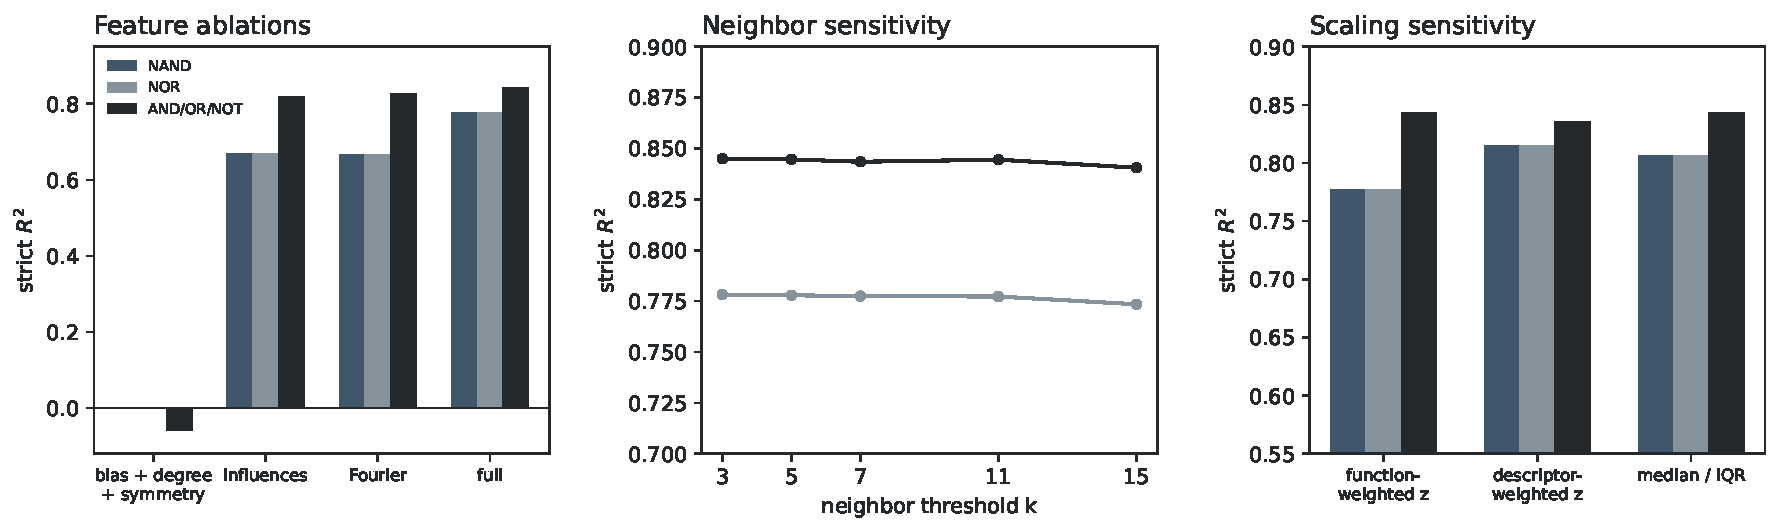
\includegraphics[width=0.99\textwidth]{../../experiments/semantic-boolean-complexity-4bit/figures/four_bit_robustness.pdf}
\caption{Feature and protocol robustness.  Across $k\in\{3,5,7,11,15\}$,
strict $R^2$ remains .773--.778 for NAND/NOR and .841--.845 for AND/OR/NOT.
Alternative scaling keeps strict $R^2$ at .806--.815 for NAND/NOR and
.836--.844 for AND/OR/NOT.}
\label{fig:robustness}
\end{figure}
\FloatBarrier

The representation languages remain distinct.  Spearman correlations of
minimum cost are .664 for NAND versus NOR and .860 for each comparison with
AND/OR/NOT.  Identical aggregate NAND/NOR prediction scores arise from their
duality and the invariant, tie-aware evaluation; their functionwise rankings
are not identical.

\section{Interpretation and limitations}

The complete four-input experiment strengthens a narrow claim: elementary,
syntax-free properties of a Boolean function contain substantial information
about exact minimal representation cost beyond input renaming, descriptor
duplication, and the matched effects of bias, degree, and symmetry.  The strict
predictor also approaches the descriptor ceiling: it recovers .777 of a
maximum .893 for NAND/NOR and .843 of .931 for AND/OR/NOT.  The result is
complementary to analytic lower-bound programs based on Fourier concentration
or related function measures \cite{lmn1993,tal2017}; it is finite, predictive,
and exact rather than an asymptotic lower bound.

It does not show that ``meaning determines difficulty.''  Identical
descriptors retain within-class cost variation, cross-language rankings are
imperfect, and changing coordinate weighting changes the exact prediction.
The universe is complete but still limited to four inputs, three related
classical bases, and a hand-designed descriptor.  Stronger follow-up tests
should use selected five-input families or exact databases, substantially
different computational models, and learned metrics evaluated under the same
fiber holdout.

\paragraph{Reproducibility.}
The checked-in experiment generates every exact target, fold, ablation,
robustness check, and all 1,000 null draws (seed 0).  It uses no model APIs or
cloud services.

\begingroup
\footnotesize
\setlength{\parskip}{0pt}
\begin{thebibliography}{9}
\setlength{\itemsep}{0pt}
\bibitem{shannon1949}
C.~E. Shannon, ``The synthesis of two-terminal switching circuits,''
\emph{Bell System Technical Journal}, 28:59--98, 1949.
\bibitem{lmn1993}
N. Linial, Y. Mansour, and N. Nisan, ``Constant depth circuits, Fourier
transform, and learnability,'' \emph{J. ACM}, 40(3):607--620, 1993.
\bibitem{odonnell2014}
R. O'Donnell, \emph{Analysis of Boolean Functions}. Cambridge University
Press, 2014; revised arXiv edition, 2021.
\bibitem{odonnellservedio2007}
R. O'Donnell and R.~A. Servedio, ``Learning monotone decision trees in
polynomial time,'' \emph{SIAM J. Comput.}, 37(3):827--844, 2007.
\bibitem{tal2017}
A. Tal, ``Formula lower bounds via the quantum method,'' in \emph{Proc. 49th
ACM STOC}, pp. 1256--1268, 2017.
\bibitem{haaswijk2020}
W. Haaswijk, M. Soeken, A. Mishchenko, and G. De Micheli, ``SAT-based exact
synthesis: Encodings, topology families, and parallelism,'' \emph{IEEE TCAD},
39(4):871--884, 2020.
\bibitem{panchu2023}
H. Pan and Z. Chu, ``Exact synthesis based on semi-tensor product circuit
solver,'' in \emph{Proc. DATE}, 2023.
\bibitem{phipson2010}
B. Phipson and G.~K. Smyth, ``Permutation $p$-values should never be zero,''
\emph{Statistical Applications in Genetics and Molecular Biology}, 9:39, 2010.
\end{thebibliography}
\endgroup

\end{document}
